\chapter{Cenni ai Sistemi Articolati}

\section{Introduzione}

\noindent Due o pi\`u corpi rigidi possono essere collegati tra loro mediante
{\em coppie rotoidali}\index{coppia!rotoidale}\footnote{In questi appunti non si descrivono le coppie rigide 
elementari; quale esempio di tali scorrimenti di superfici di corpi rigidi l'una
sull'altra citiamo la coppia rotoidale che collega le due lame delle comuni forbici
mediante un perno, precisando che le superfici combacianti sono quella del cilindro
del perno e le due superfici cilindriche dei fori che lo ospitano. Rimandiamo  il
lettore che desideri approfondire l'argomento 
a \cite{sesini1}, pagg. 22-24, o anche \cite{martin}, pagg. 9-10, o ancora
\cite{sesini3} che tratta numerosi casi di notevole interesse.}.
\noindent Le catene cinematiche che si ottengono in questo modo prendono
il nome di {\em sistemi articolati}\index{sistemi!articolati} e tale denominazione
viene mantenuta anche nei casi in cui una o pi\`u coppie rotoidali sia sostituita
da una sua degenerazione che, portando l'asse della coppia all'infinito, diventa una
{\em coppia prismatica}\index{coppia!prismatica}.
Questa vasta famiglia di meccanismi trova estese e notevolissime applicazioni:
ogni motore a combustione interna contiene almeno un sistema articolato
(il manovellismo ordinario) e svariate
sono le applicazioni dei {\em quadrilateri articolati}\index{quadrilateri!articolati} 
nelle macchine automatiche, nelle presse, nelle macchine per cucire; l'elenco
completo delle applicazioni risulterebbe molto lungo.
Esistono sistemi articolati con coppie rotoidali i cui assi sono orientati
in direzioni sghembe tra loro oppure concorrenti in un  punto 
e qualcuno di questi {\em sistemi articolati spaziali}
ha notevoli applicazioni, come il {\em giunto di Cardano}. 
La stragrande maggioranza dei sistemi articolati presenta invece coppie rotoidali
con assi tra loro paralleli. I movimenti relativi tra i vari membri si 
realizzeranno perci\`o solo in piani paralleli tra loro e ortogonali
a tali assi e questo ci permette
di identificarli come {\em sistemi articolati piani}\index{sistemi!articolati piani},
gli unici di cui accenniamo lo studio.

\noindent Dato un sistema articolato piano, senza perdita di generalit\`a, possiamo
considerare i moti piani dei suoi membri, che in realt\`a hanno sempre luogo
in piani paralleli tra loro, ma distinti, come contenuti in un solo piano. Le tracce degli assi delle coppie rotoidali che intersecano questo piano costituiscono perci\`o
un insieme di $n$ punti, tanti quanti sono gli snodi, e tali punti sono tra loro
collegati tramite $m$ corpi rigidi. Ogni punto nel piano gode di due gradi di
libert\`a di movimento, mentre i collegamenti rigidi, che mantengono invariata
la distanza tra questi punti, assorbono un grado di libert\`a ciascuno.
Ne consegue che, quando non si presentano situazioni anomale nelle quali una o 
pi\`u parti del meccanismo risulti sovra-vincolata e magari altre parti labili,
il numero di gradi di libert\`a residuo $g$ per un sistema articolato piano 
risulta essere $g=2n - m$.

\begin{figure}[hbt]
\centering
\begin{minipage}[b]{0.30\textwidth}
\centering
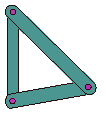
\includegraphics[width=0.8\textwidth]{part2/quadri/FIG/reticolare_triangolo.pdf}
\begin{picture}(0,0)(130,0)
\scriptsize{
\put(84,85){$n=3$}
\put(84,75){$m=3$}
\put(84,65){$g=3$}
}
\end{picture}
      \caption{\em Sistema articolato con tre coppie rotoidali e tre membri.}
 \label{fig:f_triangolo}
\end{minipage}\hfill
\begin{minipage}[b]{0.30\textwidth}
\centering
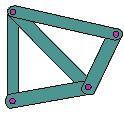
\includegraphics[width=0.8\textwidth]{part2/quadri/FIG/pentalatero.pdf}
\begin{picture}(0,0)(129,0)
        \scriptsize{
\put(82,85){$n=4$, $m=5$}
\put(82,75){$g=3$}
}
\end{picture}
        \caption{\em Sistema articolato con quattro coppie rotoidali e cinque membri.}
     \label{fig:f_pentalatero}
\end{minipage}\hfill
\begin{minipage}[b]{0.30\textwidth}
\centering
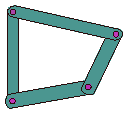
\includegraphics[width=0.8\textwidth]{part2/quadri/FIG/quadrilatero.pdf}
\begin{picture}(0,0)(129,0)
        \scriptsize{
\put(82,85){$n=4$, $m=5$}
\put(82,75){$g=4$}
}
\end{picture}
        \caption{\em Sistema articolato con quattro coppie rotoidali e quattro membri.}
     \label{fig:f_quadrilatero}
\end{minipage}
\end{figure}

\noindent In figura \ref{fig:f_triangolo} \`e riportato il pi\`u semplice sistema
articolato non banale. I gradi di libert\`a residua per tale sistema sono
$g=3\times 2- 3=3$. Tre gradi di libert\`a, nel piano, sono quelli posseduti da
qualsiasi corpo rigido svincolato, e il nostro sistema comportandosi come
un corpo indeformabile  viene classificato
e studiato nella  scienza delle costruzioni come sistema reticolare. Anche il sistema
articolato riportato in figura \ref{fig:f_pentalatero} presenta un numero di gradi
di libert\`a pari a tre. Anch'esso si comporta come un corpo rigido e fa quindi 
parte delle {\em strutture reticolari}\index{strutture reticolari}.
Il sistema riportato in figura \ref{fig:f_quadrilatero} presenta invece  $g=4$,
quindi conserva un grado di deformabilit\`a interna e per questo fa parte dei
meccanismi articolati.


\section{Quadrilateri Articolati: Velocit\`a e Accelerazioni}

\noindent Il {\em quadrilatero articolato piano}\index{quadrilateri!articolati piani}
sar\`a il solo oggetto di questa breve trattazione, in questo capitolo.
La condizione pi\`u comune \`e quella che vede
uno dei suoi quattro membri fungere da telaio: in figura
\ref{fig:f_quad_telaio} il membro $AD$ \`e il telaio. 
Il membro $BC$, sul quale non si trovano coppie rotoidali vincolate
a terra, prende il nome di {\em biella}\index{biella}. Gli altri due membri, $AB$ e $DC$, 
si chiamano {\em manovelle}\index{manovella} oppure
{\em bilancieri}\index{bilanciere} a seconda che la circostanza di potere
compiere l'intero angolo giro sia o meno verificata.

\noindent Fissato il lato che funger\`a da telaio e quindi la biella, la condizione degli
altri due membri viene determinata dalla seguente
{\em regola di Grashof}\index{Grashof, regola di}
che riportiamo pari pari e senza dimostrazione da \cite{sesini1}, pag. 99:
{\em il quadrilatero articolato piano pu\`o essere a doppia manovella o
a manovella-bilanciere,
soltanto se la somma del pi\`u piccolo e del pi\`u grande dei suoi lati non \`e
maggiore della somma degli altri due. In tal caso si ha una doppia manovella,
se l'asta fissa \`e la pi\`u corta, una manovella e un bilanciere se l'asta
fissa \`e una delle contigue alla pi\`u corta (essendo la manovella il lato pi\`u corto).
In tutti gli altri casi il quadrilatero \`e a doppio bilanciere}.

\begin{figure}[hbt]
\centering
\begin{minipage}[b]{0.48\textwidth}
\centering
     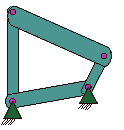
\includegraphics[width=0.88\textwidth]{part2/quadri/FIG/quadrilatero_telaio.pdf}
\begin{picture}(0,0)(170,25)
        \scriptsize{
        \put(12,169){$B$}
        \put(155,111){$C$}
        \put(132,73){$D$}
        \put(12,60){$A$}
}
\end{picture}
        \caption{\em Quadrilatero con telaio vincolato a terra.}
     \label{fig:f_quad_telaio}
\end{minipage}\hfill
\begin{minipage}[b]{0.48\textwidth}
\centering
    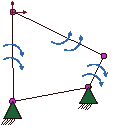
\includegraphics[width=0.88\textwidth]{part2/quadri/FIG/quadrilatero_schematico.pdf}
\begin{picture}(0,0)(170,25)
        \scriptsize{
        \put(12,169){$B$}
        \put(94,153){$\omega_{\scriptscriptstyle{BC}}$}
        \put(115,145){${\dot{\omega}}_{\scriptscriptstyle{BC}}$}
        \put(46,112){$\omega_{\scriptscriptstyle{AB}}$}
        \put(46,100){${\dot{\omega}}_{\scriptscriptstyle{AB}}$}
        \put(155,111){$C$}
        \put(148,90){$\omega_{\scriptscriptstyle{AD}}$}
        \put(142,78){${\dot{\omega}}_{\scriptscriptstyle{AD}}$}
        \put(128,72){$D$}
        \put(12,60){$A$}
}
\end{picture}
        \caption{\em Rappresentazione schematica del quadrilatero.}
     \label{fig:f_quad_schema}
\end{minipage}
\end{figure}

\noindent Ad esempio nel caso di figura \ref{fig:f_quad_telaio} abbiamo $|\overrightarrow{DC}|+|\overrightarrow{BC}|<|\overrightarrow{AB}|+|\overrightarrow{AD}|$,
quindi avremo tre possibilit\`a: due manovelle scegliendo $DC$ come telaio,
una manovella e un bilanciere quando il telaio \`e $AD$ oppure $BC$, 
infine due bilancieri con telaio $AB$. Nel caso riportato in figura
\ref{fig:f_quad_telaio}
 il telaio risulta essere
un lato contiguo al lato pi\`u corto: il membro $CD$ funger\`a, in questo
caso, da manovella
mentre il lato $AB$ sar\`a un bilanciere.



\noindent La cinematica del quadrilatero articolato si pu\`o studiare mediante le nozioni,
esposte in un capitolo precedente, circa i moti relativi. In particolare, ricordando
l'esempio di figura \ref{fig:f114} e la relativa soluzione, possiamo anche in questo caso
esprimere il moto di un membro rispetto a un riferimento fisso e a uno
mobile e imporre che le quantit\`a cinematiche coinvolte, velocit\`a e accelerazione,
corrispondano tra loro.

\noindent Riferiamoci alla rappresentazione schematica di figura
\ref{fig:f_quad_schema}, dove oltre al quadrilatero sono rappresentate velocit\`a
angolare e accelerazioni angolari della manovella $DC$ che si supporranno note.
Se ci proponessimo di trovare le analoghe grandezze cinematiche per il bilanciere $AB$,
potremmo scrivere la seguente relazione che esprime la velocit\`a del punto $C$,
sia in termini assoluti, sia in termini relativi, nel suo moto attorno al
punto $B$. Qui immaginiamo incardinato il sistema di riferimento relativo che
trasla, mantenendo perci\`o i suoi assi sempre nelle medesime direzioni.
Avremo
\begin{equation}
{\bm v}_{\scriptscriptstyle{{\rm ass}}}=
{\bm v}_{\scriptscriptstyle{{\rm rel}}}+
{\bm v}_{\scriptscriptstyle{{\rm tr}}}\,,
\label{eq:e_v_rivals_q}
\end{equation}
\noindent cio\`e
\begin{equation}
{{\bm v}_{\scriptscriptstyle{C}}}=
{{\bm v}_{\scriptscriptstyle{C}}}_{\scriptscriptstyle{{\rm rel}}}+
{{\bm v}_{\scriptscriptstyle{B}}}\,.
\label{eq:e_v_quad_schematico}
\end{equation}
\noindent Riferendoci alle quantit\`a indicate in figura \ref{fig:f_quad_schema},
possiamo riscrivere la \ref{eq:e_v_quad_schematico} nel modo seguente
\begin{equation}
{{\bm v}_{\scriptscriptstyle{C}}}=
\omega_{\scriptscriptstyle{BC}} |\overrightarrow{BC}| \widehat{{\perp{BC}}}
+\omega_{\scriptscriptstyle{AB}} |\overrightarrow{AB}| \widehat{{\perp{AB}}}\,,
\label{eq:e_v_quad_schematico0}
\end{equation}
\noindent dove i versori
$\widehat{{\perp{BC}}}$ e $\widehat{{\perp{AB}}}$ indicano che la direzione dei
due termini incogniti a destra del segno di uguaglianza \`e nota.
L'equazione \ref{eq:e_v_quad_schematico0} contiene pertanto due 
termini vettoriali di modulo incognito e direzione conosciuta.
Si pu\`o dunque seguire (in linea di principio) lo schema grafico riportato in figura
\ref{fig:f116}, e lo svolgimento riportato nel medesimo contesto che ci permette 
di determinare la velocit\`a angolare del bilanciere e della biella,
$\omega_{\scriptscriptstyle{AB}}$ e $\omega_{\scriptscriptstyle{BC}}$.

\noindent Consideriamo ora le accelerazioni. Dato che il sistema di riferimento relativo trasla, scrivendo la \ref{e138} il termine dell'accelerazione di Coriolis sar\`a assente:
\begin{equation}
{{\bm a}_{\scriptscriptstyle{C}}}=
{{\bm a}_{\scriptscriptstyle{C}}}_{\scriptscriptstyle{{\rm rel}}}+
{{\bm a}_{\scriptscriptstyle{B}}}\,.
\label{eq:e_a_quad_schematico}
\end{equation}
\noindent Risulta conveniente scrivere i termini
${{\bm a}_{\scriptscriptstyle{C}}}_{\scriptscriptstyle{{\rm rel}}}$ e 
${{\bm a}_{\scriptscriptstyle{B}}}$ 
come somma delle loro
componenti: normale e tangenziale
\begin{equation}
{{\bm a}_{\scriptscriptstyle{C}}}=
-\omega^2_{\scriptscriptstyle{BC}} \overrightarrow{BC} + {\dot{\omega}_{\scriptscriptstyle{BC}}}|\overrightarrow{BC}|\widehat{{\perp{BC}}}
-\omega^2_{\scriptscriptstyle{AB}} \overrightarrow{AB} + {\dot{\omega}_{\scriptscriptstyle{AB}}}|\overrightarrow{AB}|\widehat{{\perp{AB}}}\,,
\label{eq:e_a_quad_schematico2}
\end{equation}
\noindent dove, ancora una volta, i versori
$\widehat{{\perp{BC}}}$ e $\widehat{{\perp{AB}}}$ indicano che la direzione
di questi due termini incogniti \`e conosciuta.
Gli altri termini risultano essere tutti noti, quindi
ricadiamo ancora nel caso di una equazione vettoriale dove le incognite sono
i moduli del secondo e del quarto termine a destra del segno di uguaglianza della
\ref{eq:e_a_quad_schematico2} e per la soluzione ci riferiamo, una volta di pi\`u,
al procedimento di figura \ref{fig:f116}, dal quale
otterremo anche
${\dot{\omega}}_{\scriptscriptstyle{AB}}$ e ${\dot{\omega}}_{\scriptscriptstyle{BC}}$.

\section{Applicazioni dei Quadrilateri} \label{q_squilibrio}
\noindent Abbiamo gi\`a ricordato che il quadrilatero articolato si presta a
svariatissime applicazioni. Nella sua versione con doppia manovella esso
pu\`o trasmettere il moto rotatorio
tra due alberi paralleli, nella configurazione in cui
le tracce degli assi di tali alberi siano i centri delle
rispettove coppie rotoidali sul telaio. In questo caso,
se il quadrilatero presenta i lati opposti uguali tra loro, la trasmissione
del moto sar\`a {\em omocinetica}\index{trasmissione!omocinetica} con
rapporto di trasmissione unitario e il meccanismo
prende il nome di {\em parallelogramma articolato}\index{parallelogramma articolato},
famoso per aver collegato, un tempo, le ruote delle locomotive a vapore in
modo tale da renderle tutte motrici.
La trasmissione del moto tramite un quadrilatero generico non sar\`a pi\`u,
in generale, omocinetica
e si potranno avere due casi di particolare interesse: manovella-manovella, oppure
manovella-bilanciere. In entrambi i casi, il progetto (sintesi) del quadrilatero
mira a ottenere un particolare movimento rotatorio o oscillatorio 
sulla manovella o sul bilanciere in uscita, tale da rendere diverse tra loro
 le velocit\`a di
percorrenza ciclica delle due fasi che questo membro attraversa durante il moto
a velocit\`a angolare costante della manovella motrice.

\begin{figure}[hbt]
\centering
\begin{minipage}[b]{0.48\textwidth}
\centering
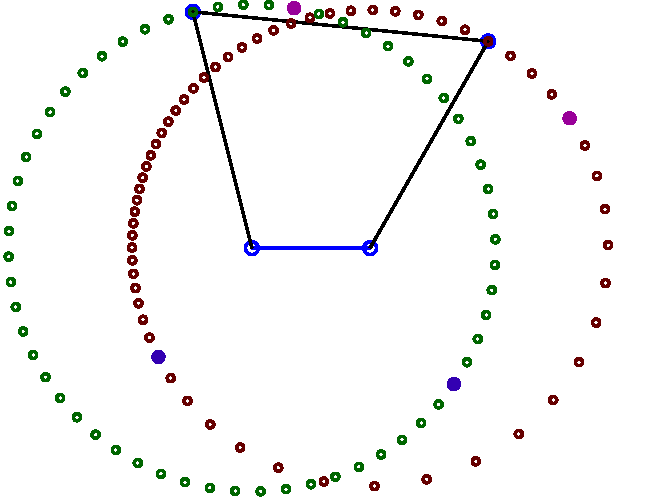
\includegraphics[width=0.9\textwidth]{part2/quadri/FIG/quadri/doppia_manovella.pdf}
\begin{picture}(0,0)(130,0)
\scriptsize{
\put(39,125){$\alpha_2=81^{\circ}$}
\put(8,119){$B$}
\put(88,114){$C$}
\put(26,53){$A$}
\put(55,53){$D$}
\put(85,26){$\alpha_1=333^{\circ}$}
\put(109,97){$\beta_2=34^{\circ}$}
\put(11,37){$\beta_1=214^{\circ}$}
}
\end{picture}
      \caption{\em Quadrilatero a doppia manovella.}
 \label{fig:doppia_manovella}
\end{minipage}\hfill
\begin{minipage}[b]{0.48\textwidth}
\centering
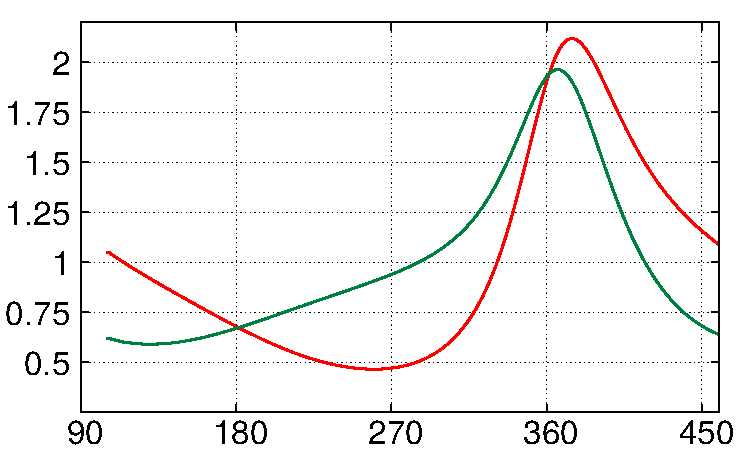
\includegraphics[width=0.9\textwidth]{part2/quadri/FIG/quadri/vel_doppia_manovella.pdf}
\vspace*{6mm}
\begin{picture}(0,0)(129,0)
\scriptsize{
\put(-5,42){${\omega_{\scalebox{.5}{DC}}}/{\omega_{\scalebox{.5}{AB}}}$}
\put(45,60){${\omega_{\scalebox{.5}{BC}}}/{\omega_{\scalebox{.5}{AB}}}$}
\put(124,2){$\alpha$}
}
\end{picture}
\vskip .5mm
      \caption{\em Velocit\`a angolare della manovella $CD$ e della biella $BC$.}
     \label{fig:vel_doppia_manovella}
\end{minipage}
\end{figure}

\noindent La figura \ref{fig:doppia_manovella} riporta un quadrilatero con doppia
manovella: $AB$ e $CD$ compiono intere rotazioni, mentre l'asta $BC$ funge da biella.
In tale figura sono riportate alcune posizioni occupate dalle cerniere $B$ e $C$ 
durante la rotazione a velocit\`a angolare costante della manovella $AB$.
Analizzando tali posizioni si nota che la spaziatura dei punti
generati dalla cerniera $B$, che \`e l'estremo della manovella motrice, \`e appunto
costante mentre la spaziatura delle tracce relative alla cerniera $C$, che \`e l'estremo
della manovella condotta, \`e variabile.
Ci\`o rende perfettamente conto delle velocit\`a angolari delle due manovelle:
come abbiamo detto, costante per quella motrice e variabile per la manovella cedente.
La figura \ref{fig:vel_doppia_manovella} riporta la velocit\`a angolare della manovella
$CD$ e, per completezza-curiosit\`a, quella della biella $BC$, rapportate alla
velocit\`a angolare della manovella motrice. 

\noindent La velocit\`a angolare variabile della manovella $DC$ pu\`o essere a
sua volta utilizzata per azionare un secondo meccanismo come, ad esempio, il 
manovellismo ordinario di una pressa, al quale sarebbe in tal modo possibile
un funzionamento con {\em ritorno rapido}\index{ritorno rapido}.
Consideriamo infatti l'ipotesi di muovere quest'ultimo manovellismo mediante la rotazione della
manovella $DC$ (che fisicamente potrebbe coincidere in parte con quella del manovellismo
stesso). Scegliendo opportunamente la posizione del punto morto di tale manovellismo,
cio\`e il punto di partenza per gli angoli di manovella, potremmo avere, per il
cursore del manovellismo mosso, una corsa di andata pi\`u lenta rispetto a quella di
ritorno o viceversa.
Con riferimento alla figura \ref{fig:doppia_manovella} scegliamo come angolo di
partenza $\beta_1$. Il cursore del manovellismo invertir\`a il suo moto in $\beta_2$,
distante $180^{\circ}$ da $\beta_1$, a valle di una rotazione della
manovella $AB$ di un angolo di ``andata'' pari a
$\alpha_a=\alpha_2-\alpha_1$. Parimenti, il movimento di ritorno si estender\`a
sull'arco percorso sempre di $AB$ pari a
$\alpha_r=360-(\alpha_2-\alpha_1)$.
I tempi di andata e di ritorno, $t_a$ e $t_r$, saranno perci\`o diversi tra loro
e proporzionali ai due angoli percorsi dalla manovella motrice durante le
rispettive fasi:
\begin{equation}
\alpha_a = 360^{\circ} {t_a \over{t_a+t_s}}\,,\;\;\;
\alpha_r = 360^{\circ} {t_s \over{t_a+t_s}}\,.
\label{eq:angoli_andata_ritorno}
\end{equation}
\noindent Il rapporto $s={{\alpha_a}\over{\alpha_r}}$ 
viene talvolta indicato come {\em squilibrio del quadrilatero}\index{quadrilatero!squilibrio}
e, come abbiamo gi\`a accennato, dipende anche dalla scelta della
 posizione iniziale
$\alpha_1$. Lo squilibrio si ritiene tanto pi\`u elevato quanto pi\`u
esso si scosta dall'unit\`a.
In pratica, accade raramente che 
il rapporto tra gli angoli di andata e ritorno, cio\`e lo squilibrio, sia maggiore di
tre o minore di un terzo.
In figura \ref{fig:doppia_manovella} sono indicate le coppie di angoli
$\alpha_1$, $\beta_1$, $\alpha_2$, $\beta_2$ che per questo quadrilatero
realizzano il {\em massimo squilibrio}:
\begin{equation}
s={{333^{\circ}-81^{\circ}}\over{360^{\circ} -333^{\circ} +81^{\circ}}} = 2.3\,.
\label{eq:esempio_squilibrio}
\end{equation}
\noindent Evidenziamo, sperando di contribuire in modo positivo alla chiarezza dell'argomento,
che esiste sempre la
possibilit\`a di scegliere l'inizio delle rotazioni della manovella $DC$, $\beta_1$,
in modo tale da rendere lo squilibrio minimo, cio\`e pari a uno. Con dubbia 
utilit\`a pratica, vedremo in tal caso compiere
alla manovella cedente un mezzo giro dopo che la motrice ha compiuto anch'essa $180^{\circ}$,
rimanendo tuttavia variabile il rapporto di trasmissione tra le due manovelle.
\begin{figure}[hbt]
\centering
\begin{minipage}[b]{0.48\textwidth}
\centering
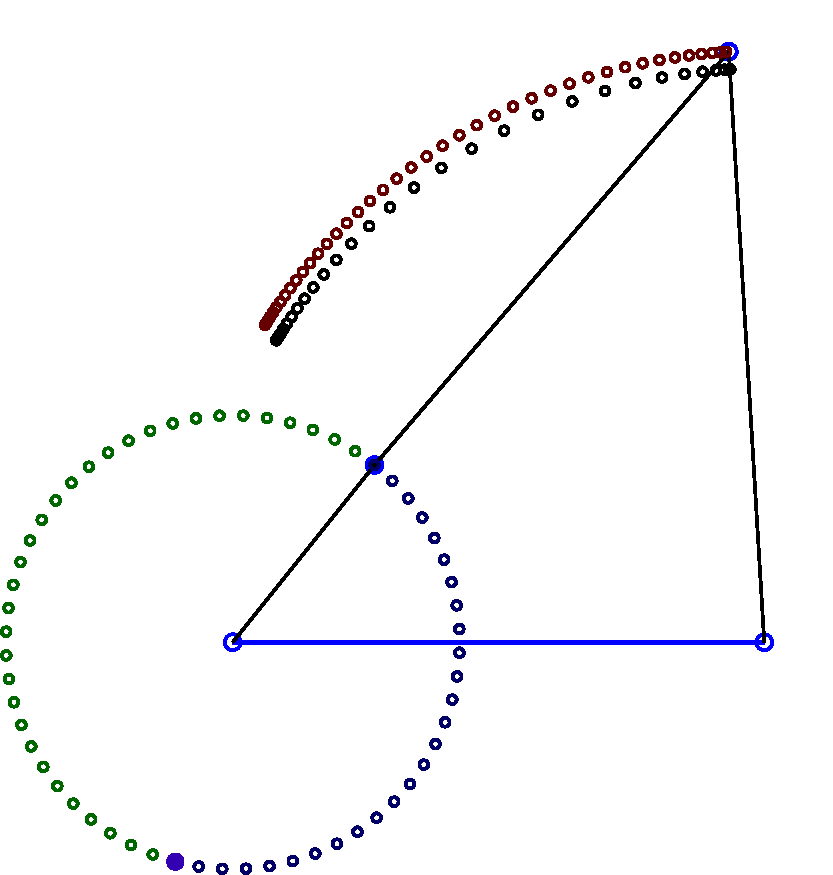
\includegraphics[width=0.9\textwidth]{part2/quadri/FIG/quadri/manovella_bilanciere.pdf}
\begin{picture}(0,0)(130,0)
\scriptsize{
\put(110,152){$C$}
\put(35,83){$B$}
\put(46,75){$\alpha_1=51^{\circ}$}
\put(8,34){$A$}
\put(111,34){$D$}
\put(4,-6){$\alpha_2=263^{\circ}$}
}
\end{picture}
\vskip 2mm
      \caption{\em Quadrilatero a manovella e bilanciere.}
 \label{fig:manovella_bilanciere}
\end{minipage}\hfill
\begin{minipage}[b]{0.48\textwidth}
\centering
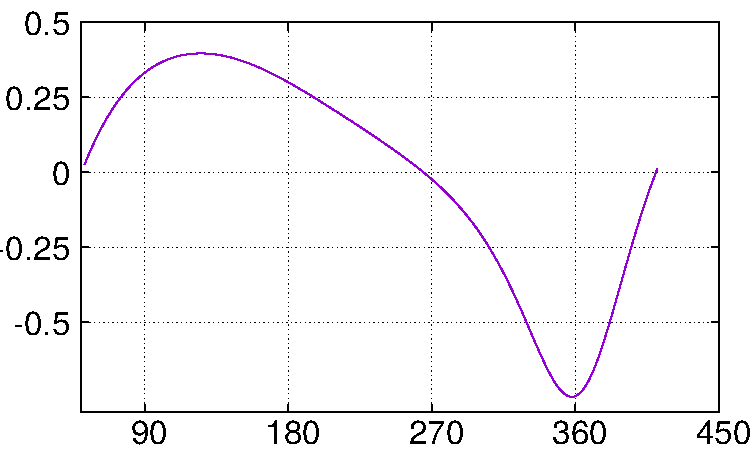
\includegraphics[width=0.9\textwidth]{part2/quadri/FIG/quadri/vel_manovella_bilanciere.pdf}
\vspace*{6mm}
\begin{picture}(0,0)(129,0)
\scriptsize{
\put(35,75){${\omega_{\scalebox{.5}{DC}}}/{\omega_{\scalebox{.5}{AB}}}$}
\put(127,2){$\alpha$}
}
\end{picture}
\vskip 2mm
      \caption{\em Velocit\`a angolare della manovella $CD$.}
     \label{fig:vel_manovella_bilanciere}
\end{minipage}
\end{figure}
\noindent In figura \ref{fig:manovella_bilanciere} \`e rappresentato un quadrilatero il cui
membro $DC$ non compie intere rotazioni ma oscilla percorrendo archi di $54.2^{\circ}$  che, anche in questo esempio, assumono i nomi di andata e ritorno.
Nella stessa figura sono evidenziate, tramite la traccia della cerniera $C$, 
le differenti velocit\`a con le quali vengono descritti tali archi.
Anche qui i tempi di percorrenza
dell'andata e del ritorno, $t_a$ e $t_b$, saranno proporzionali ai corrispondenti
angoli percorsi,
a velocit\`a costante, dalla manovella $AB$. Perci\`o, appoggiandoci 
alle precedenti notazioni,
lo squilibrio di questo quadrilatero diventa
\begin{equation}
s={{263^{\circ}-51^{\circ}}\over{360^{\circ} -263^{\circ} +51^{\circ}}} = 1.43\,.
\label{eq:squilibrio_manovella_bilanciere}
\end{equation}
\noindent In questo caso, gli angoli sottesi dal bilanciere nei quali avviene
l'inversione della sua corsa
risultano  inequivocabili e lo squilibrio massimo,
riportato nella \ref{eq:squilibrio_manovella_bilanciere},
\`e l'unico squilibrio del quale abbia senso parlare.

\noindent Interessanti applicazioni di meccanismi con tempi di andata e ritorno diversi
tra loro si possono realizzare mediante l'impiego di particolari quadrilateri nei
quali una coppia rotoidale ha asse improprio. Tali meccanismi si chiamano {\em manovellismi}\index{manovellismo} e, 
data la loro importanza e diffusione, verranno trattati nel successivo
capitolo, a loro completamente dedicato.

\noindent Il problema di ottenere particolari quadrilateri, a doppia manovella oppure a manovella e bilanciere, che realizzino un dato squilibrio tra i tempi di andata e 
ritorno pu\`o essere risolto tramite specifici metodi
grafici i quali, se coadiuvati da una buona dose di esperienza del progettista,
portano al risultato desiderato.
A tali metodi di sintesi non facciamo cenno, ritenendoli
fuori luogo in questi appunti e ottimamente collocati in libri specialistici come il
pluricitato \cite{ruggieri}, pagg. 215--220. Aggiungiamo che la sintesi dei quadrilateri
avviene molto frequentemente tramite analisi ripetute, partendo da geometrie iniziali
che solitamente il progettista porta con s\'e nel suo bagaglio di esperienza.

\section{Curve di Biella}

\noindent Fin qui, poco si \`e detto del moto della biella eccezion fatta per la 
figura \ref{fig:vel_doppia_manovella} dove \`e riportata la velocit\`a angolare
della biella $BC$ rapportata a quella della manovella $AB$.
D'altra parte lo studio del moto della biella di un quadrilatero articolato ha
applicazioni pratiche molto rilevanti.
Per un dato quadrilatero, i punti del piano su cui giace la
biella (pensato solidale con essa) percorrono, durante il movimento di questa, una doppia infinit\`a di curve.
Al variare del {\em punto di biella}\index{biella!punto di} considerato, tali
{\em curve di biella}\index{biella!curve di} assumono forme diversissime tra loro
e possono risultare appetibili quando appunto servono movimentazioni
cicliche e peculiari.
Le curve di biella presentano infatti una grande
variet\`a di archi e intrecci
e vengono spesso prese in considerazione in diversi contesti
del progetto di macchine automatiche.
In tempi passati, il progettista interessato all'impiego di una curva di biella
si affidava per la sua scelta ai cosiddetti {\em atlanti}\index{atlanti di quadrilateri}.
Tra queste opere, la pi\`u
completa \`e quella di Hrones e Nelson \cite{hrones}, che presenta, tramite
un ingegnoso ordine sistematico, pi\`u di settemila curve di biella.  
\begin{figure}[hbt]
\centering
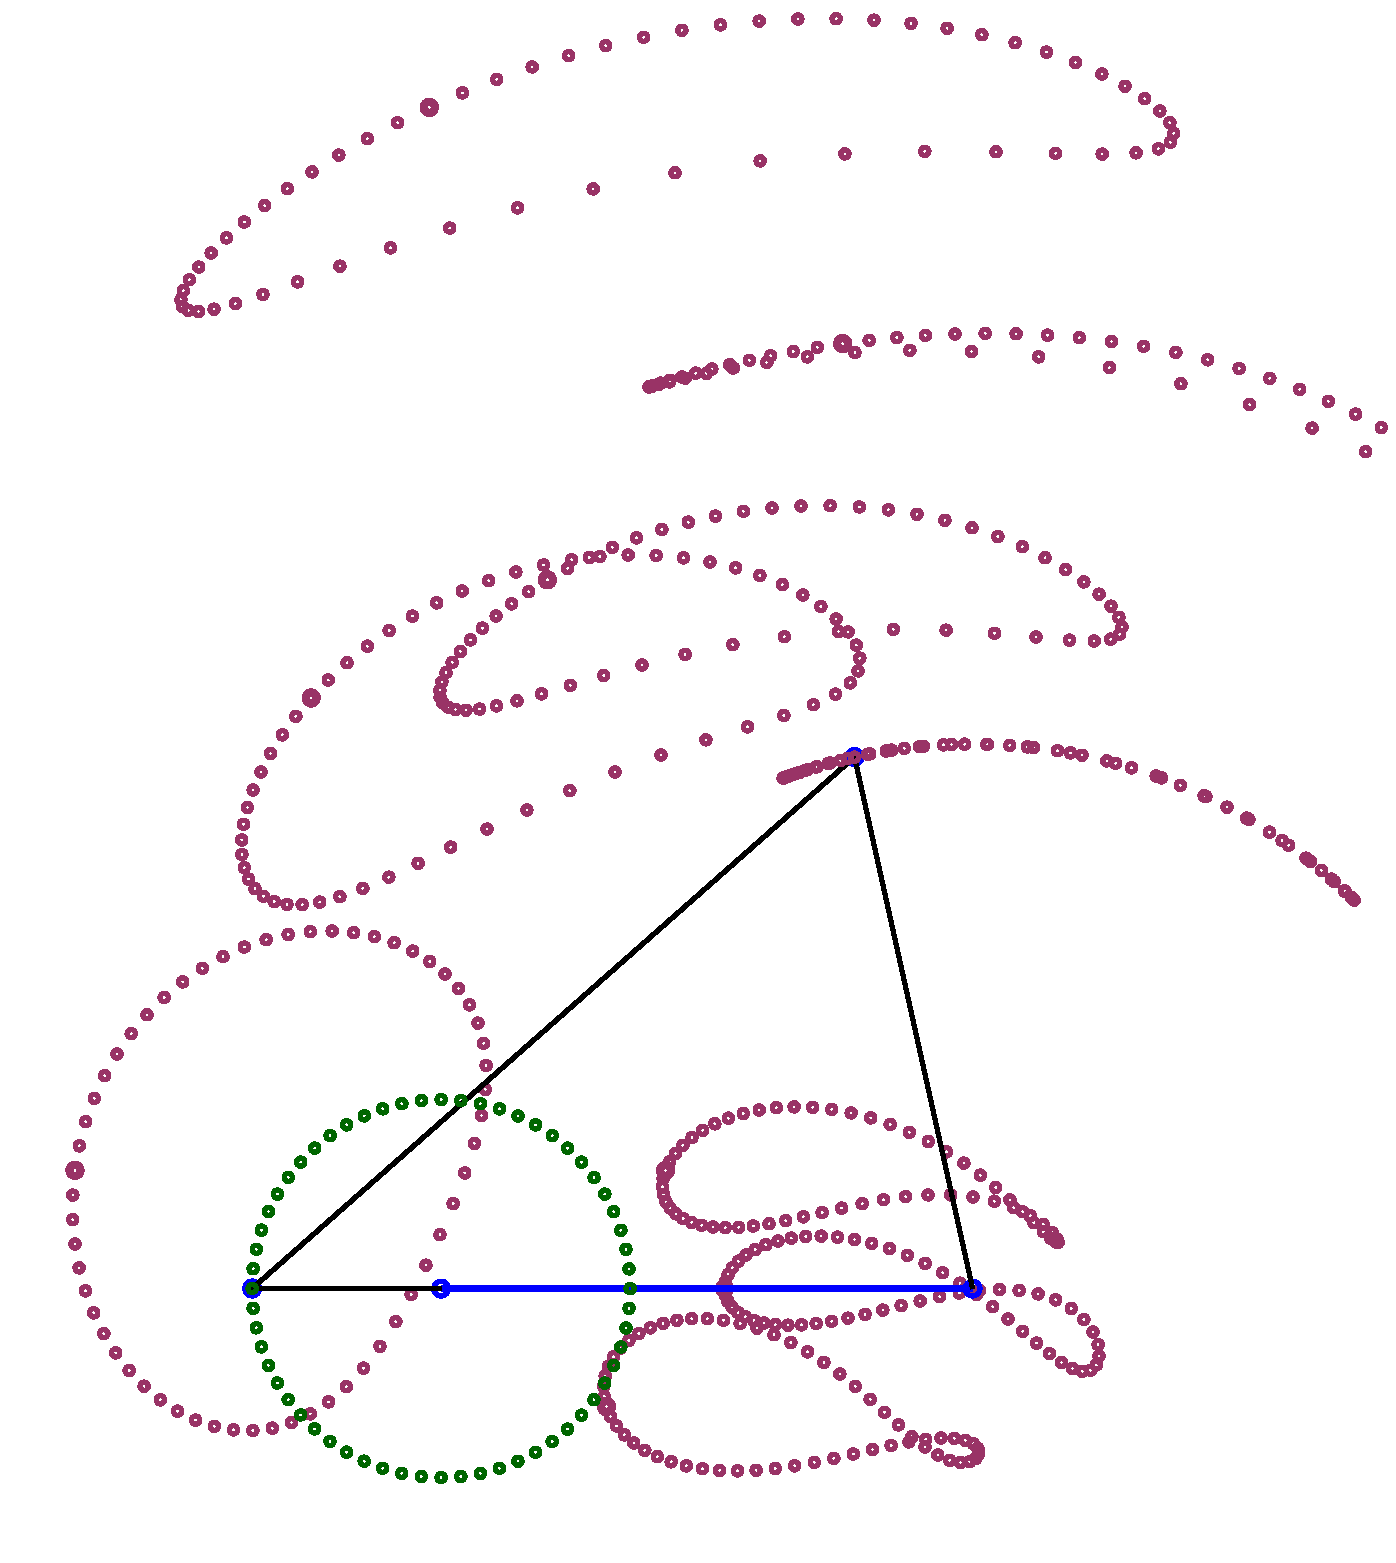
\includegraphics[width=0.9\textwidth]{part2/quadri/FIG/quadri/curve_di_biella.pdf}
\begin{picture}(0,0)(250,0)
\scriptsize{     
\put(10,352){\rotatebox{-54}{$\longrightarrow$}}
\put(-13,354){punto di biella}
\put(107,298){\rotatebox{-54}{$\longrightarrow$}}
\put(83,301){punto di biella}
\put(125,182){$C$}
\put(22,54){$A$}
\put(-30,54){$B$}
\put(142,54){$D$}
}
\end{picture}
      \caption{\em Alcune curve di biella di un quadrilatero articolato manovella-bilanciere. I punti di biella sono evidenziati.}
 \label{fig:f_cur_biella}
\end{figure}

\noindent Oggigiorno,  non \`e difficile trovare ``pagine di calcolo'' che contengono
analizzatori di 
quadrilateri i quali, a fronte dei dati che identificano il meccanismo da
studiare e della scelta del punto di biella, forniscono immediatamente la 
relativa curva. Il progettista, guidato dall'esperienza e dalle analisi numeriche
ripetute, pu\`o cos\`i
avvicinarsi per passi alla soluzione del proprio problema di progetto.
Naturalmente esistono interi programmi commerciali di calcolo che possono analizzare
i quadrilateri articolati, i quali programmi spesso sono molto generali e pensati
per l'analisi di meccanismi anche molto complessi.
Diciamo per\`o, per esperienza, che un tecnico, qualora si accinga all'utilizzo
delle curve di biella, difficilmente rinuncia a trarre ispirazione dai casi
riportati sugli atlanti, se non altro per generare l'embrione di quello che poi
costituir\`a la soluzione finale. 
\begin{wrapfigure}{r}{0.5\textwidth}
     \begin{center}
     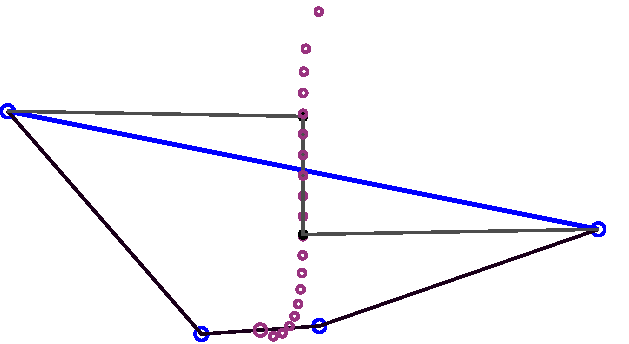
\includegraphics[width=0.42\textwidth]{part2/quadri/FIG/quadri/watt.pdf}
     \end{center}
\begin{picture}(0,0)(0,0)
        \scriptsize{
        \put(77,85){$B$}
        \put(58,18){$B'$}
        \put(90,45){$C$}
        \put(90,20){$C'$}
        \put(89,69){$E$}
        \put(73,19){$E'$}
        \put(155,58){$D$}
        \put(11,73){$A$}
}
\end{picture}
        \caption{\em Quadrilatero di {\em Watt}.}
     \label{fig:watt}
\end{wrapfigure}
\noindent A titolo di esempio riportiamo in figura \ref{fig:f_cur_biella}
le traiettorie di alcuni punti di biella del quadrilatero a manovella-bilanciere
$ABCD$. Anche in questo caso, la distanza
tra le tracce lasciate dal punto di biella d\`a un'idea precisa della 
velocit\`a mediante la quale tale punto percorre la propria traiettoria
(accorgimento grafico, questo,
riportato con precisione sugli atlanti tramite linee a tratteggio di lunghezza
diversificata).
\noindent Non deve sorprendere se particolari curve
di biella, che, da un punto di vista teorico, rettilinee non sono, vengano
invece sfruttate nella pratica come generatori di spostamenti rettilinei
o {\em guide rettilinee
approssimate}\index{guide rettilinee approssimate}.
La figura \ref{fig:watt} mostra una di queste guide approssimata dal
movimento del
punto centrale $E$ della biella $BC$. Il quadrilatero $ABCD$ prende il nome dal suo 
inventore e si chiama quadrilatero di {\em Watt} (talvolta parallelogramma
di {\em Watt}, anche se le applicazioni che lo vedono
in tal veste sono molto rare).
Nella nostra figura, le tracce del punto di biella $E$ non sono equidistanziate,
infatti la figura \`e stata ottenuta
mediante il movimento a velocit\`a costante del bilanciere $AB$;
inoltre, sempre nella figura citata, viene riportato un pezzo
molto esteso della curva che il punto $E$ pu\`o percorrere.
Normalmente per\`o questo meccanismo viene
impiegato sfruttando la guida rettilinea approssimata, fornita dal punto mediano della 
biella, a fronte di un azionamento
direttamente applicato allo stesso punto $E$.
Tale azionamento pu\`o essere l'oscillazione verticale del telaio di un'automobile
quando, ad esempio, il quadrilatero di Watt viene utilizzato nelle sospensioni.
Ma il movimento oscillatorio verticale della scocca di un veicolo
\`e limitato nella propria corsa dai vincoli geometrici della sospensione
stessa, pertanto va da s\'e che il punto di biella percorrer\`a
soltanto una porzione, quella quasi rettilinea, della
 sua traiettoria possibile.
\newpage
\thispagestyle{empty}
\null

\endinput 
\section{Cenni Generali sulla Sintesi dei Quadrilateri}
\noindent Desideriamo concludere questo paragrafo con un brevissimo cenno
riassuntivo alle tecniche di sintesi del quadrilatero articolato.
Per prima cosa distinguiamo da subito due strade possibili: quella {\em diretta}\index{
sintesi diretta dei quadrilateri} e quella {\em indiretta}\index{sintesi
indiretta dei quadrilateri}. La prima di queste strade conduce alla determinazione,
tramite metodi grafici o analitici, dei punti di cerniera del quadrilatero
che soddisfa le richieste di
progetto in modo univoco oppure ad infinit\`a di soluzioni dipendenti da uno o 
pi\`u parametri liberi, come potrebbero essere il fattore di scala o il posizionamento
di una o pi\`u cerniere.
Il metodo indiretto consiste invece nell'analisi numerica ripetuta di diverse
soluzioni che,
guidata dall'intuito e dall'esperienza del progettista, nonch\'e dalle agili
possibilit\`a interattive dei moderni programmi di calcolo, porta via via alla
soluzione ottimale. 
\`E possibile una classificazione sistematica dei vari problemi di sintesi
che possono essere ricondotti a tre problemi paradigmatici.

\noindent Il primo di questi problemi \`e gi\`a stato esposto, con piglio descrittivo,
poco sopra in queste note. Si tratta, con riferimento alle figure
\ref{fig:doppia_manovella} o \ref{fig:manovella_bilanciere}, di correlare le posizioni
angolari della manovella motrice con le rispettive posizioni dell'altra manovella
(oppure bilanciere). Si parla in questi casi di uso del quadrilatero come
{\em generatore di funzioni}\index{generatore di funzioni}. Crediamo sia evidente
che non si possa sperare di ottenere un meccanismo in grado di seguire
pedissequamente una data funzione arbitraria $\beta(\alpha)$. Siccome le incognite,
o gradi di libert\`a,
risultano essere le quattro lunghezze dei membri del quadrilatero \`e ragionevole
aspettarsi che potranno essere soddisfatte puntualmente soltanto quattro valori:
$\beta(\alpha_1)$, $\beta(\alpha_2)$, $\beta(\alpha_3)$ e $\beta(\alpha_4)$.
In questo caso quindi vengono fatte corrispondere cinque posizioni del quadrilatero e 
si parla di problema a dieci gradi di libert\`a.
Anzich\'e essere fatte valere tutte sugli angoli, queste quattro condizioni potrebbero,
in parte, essere  applicate alle
derivate di tali angoli: ad esempio, nella sintesi del quadrilatero di figura
\ref{fig:manovella_bilanciere} dovremmo imporre velocit\`a nulla nelle due posizioni
di {\em punto morto}\index{punto morto} del bilanciere $DC$ e avremo cos\`i assegnate
$\beta(\alpha_1)$, ${\dot\beta}(\alpha_1)=0$, $\beta(\alpha_2)$ e ${\dot\beta}(\alpha_2)=0$. 
\noindent Un altro tipico problema di sintesi pu\`o essere ricondotto alla ricerca 
di traiettorie desiderabili per un dato punto del {\em piano di biella}\index{biella!piano di}, traiettorie
cio\`e percorse da un punto di biella. Ci siamo gi\`a occupati di queste traiettorie,
in modi descrittivo, in un paragrafo precedente e potremmo, in linea con la maggior parte
degli autori che trattano questo argomento, chiamare questa funzione richiesta al
quadrilatero {\em generazione di traiettorie}\index{generazione!di traiettorie}.
Da un punto di vista molto formale si potrebbe asserire che, in questo caso,
le incognite
saranno le quattro coordinate delle cerniere del telaio, le tre lunghezze delle
aste rimanenti, le due lunghezze dei rimanenti lati del triangolo che individua (tramite
uno dei suoi vertici) il punto di biella e infine la posizione iniziale della 
manovella movente: totale 10 gradi di libert\`a. A questi gradi di libert\`a,
sempre molto formalmente, corrisponderanno cinque posizioni (due coordinate ciascuna)
che potranno essere soddisfatte, oppure quattro posizioni e una tangente alla curva
di biella in uno dei quattro punti, oppure tre punti e due tangenti.
 
\noindent Un terzo problema di sintesi riguarda la possibilit\`a di fare guidare alla
biella un oggetto da posizionare nel piano. Questa funzione si pu\`o chiamare 
{\em generazione di moti piani}\index{generazione!di moti piani}. Anche qui, 
\cite{ruggieri}, pag. 279, i gradi di libert\`a sono dieci e si potrebbero soddisfare
cinque posizioni per l'oggetto movimentato, che saturerebbero tutte le incognite.

\noindent I tre problemi di sintesi dimensionale del quadrilatero sono per\`o tutti
riconducibili l'uno all'altro come riportato in \cite{ruggieri} pag 279.
Ci sembra opportuno dare solo un brevissimo cenno alla soluzione al terzo di questi
problemi a 5 gradi di libert\`a (o dieci se si considera che ogni punto \`e individuato
da due coordinate. La generazione di particolari posizioni della biella \`e stato
formulato, in modo assai generale, da Burmester quindi tale problema ne prende il
nome.

\noindent Nella sua formulazione pi\`u generale, il {\em problema di Burmester}
consiste nell'individuare un quadrilatero che,  tramite un punto di biella, tocchi
alcune posizioni precise.
Doverebbe essere chiaro da quanto fin qui esposto che il numero massimo di tali punti
di precisione non pu\`o superare il numero cinque. 
Difficilmente per\`o ci si pu\`o spingere alla saturazione di tutti i gradi di
libert\`a disponibili, in quanto si potrebbero trovare soluzioni non praticabili.
Ci si accontenta spesso di progettare quadrilateri in cui un punto di biella 
passa per tre punti di precisione, lasciando liberi due gradi di libert\`a in modo
da individuare, nel novero delle soluzioni ottenute,
meccanismi effettivamente realizzabili.

\noindent Sebbene gli studi del Burmester siano molto interessanti e
indispensabili laddove venga
richiesto al punto di biella il passaggio da quattro o da cinque punti di
precisione,
facciamo semplicemente notare che la soluzione per tre soli punti di precisione
\`e talmente a portata di mano che sarebbe un peccato non descriverla.

\noindent Sia dunque da realizzare un quadrilatero in cui un punto di biella
passi da tre punti stabiliti. Per tali punti passer\`a una e una sola circonferenza.
Il moto della biella avr\`a quindi come centro di spostamento finito il centro
di tale circonferenza.
(da concludere)

